% !TeX document-id = {d3180326-e0d2-447c-ac39-50b0271e3b1b}
% 固定の資料フォルダ。以後の修正はこの main.tex を直接編集する。
\documentclass[a4paper,uplatex,dvipdfmx]{jsarticle}
\usepackage[haranoaji,unicode]{pxchfon}
\usepackage[dvipdfmx]{graphicx,color}
\usepackage{amsmath,amssymb,xurl,multicol,caption}
\usepackage[dvipdfmx,unicode]{hyperref}
\usepackage{pxjahyper}
\captionsetup{font=small,labelfont=normalfont,labelsep=quad,hypcap=false}
\raggedbottom
\raggedcolumns
\hypersetup{hidelinks,pdftitle={進捗報告},pdfauthor={M1 TANG YU}}
\topmargin=-2.0cm
\textheight=25.0cm
\textwidth=17.0cm
\oddsidemargin=-1.0cm
\evensidemargin=-1.0cm
\renewcommand{\baselinestretch}{0.95}
\setlength{\columnsep}{7mm}
\setlength{\multicolsep}{6pt}
\makeatletter
\renewcommand{\subsection}{\@startsection{subsection}{2}{\z@}%
  {.7\Cvs}{.25\Cvs}{\normalfont\normalsize\headfont}}
\setlength{\@fptop}{0pt}
\setlength{\@dblfptop}{0pt}
\renewcommand{\@maketitle}{%
  \begin{center}
    {\Large\@title\par}
    \vspace{0.4em}
    {\normalsize\@author\par}
    \vspace{0.2em}
    {\normalsize\@date\par}
  \end{center}
  \vspace{0.3em}}
\makeatother
\newcommand{\degc}{^{\circ}}
\newcommand{\talkpoint}[1]{\par\smallskip\noindent\textbf{#1}\par}
\title{\textbf{進捗報告}}
\author{M1 TANG YU}
\date{2026年11月2日}

\begin{document}
\maketitle
\setlength{\abovedisplayskip}{5pt}
\setlength{\belowdisplayskip}{5pt}
\setlength{\abovedisplayshortskip}{3pt}
\setlength{\belowdisplayshortskip}{3pt}

\noindent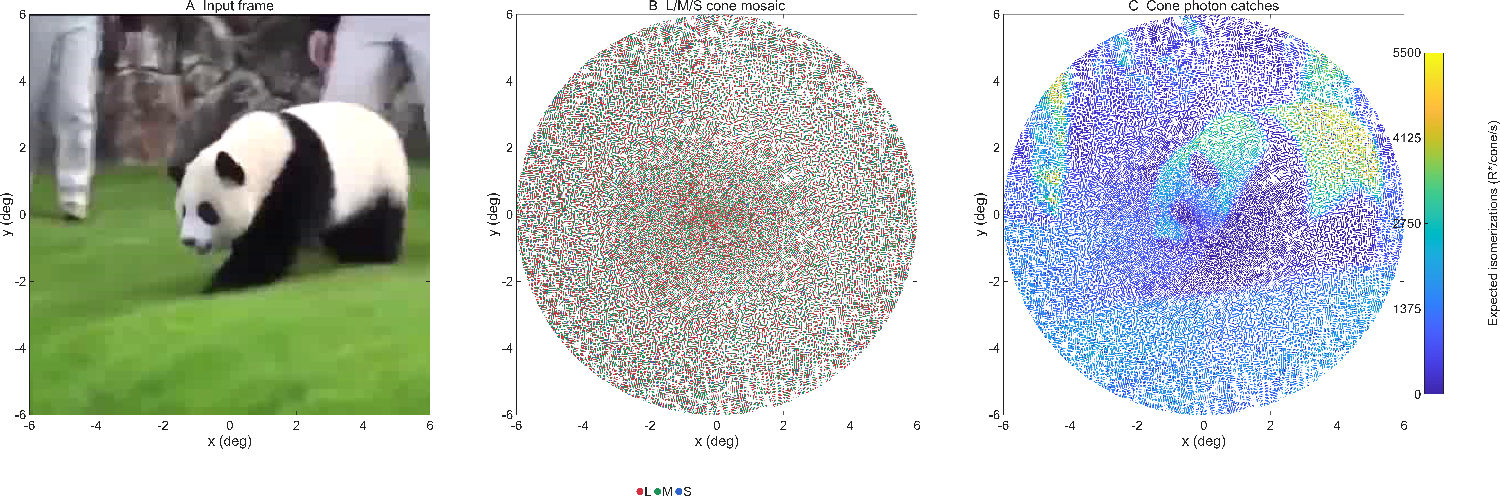
\includegraphics[width=\linewidth]{isetbio_cone_distribution.pdf}\par
\smallskip
\noindent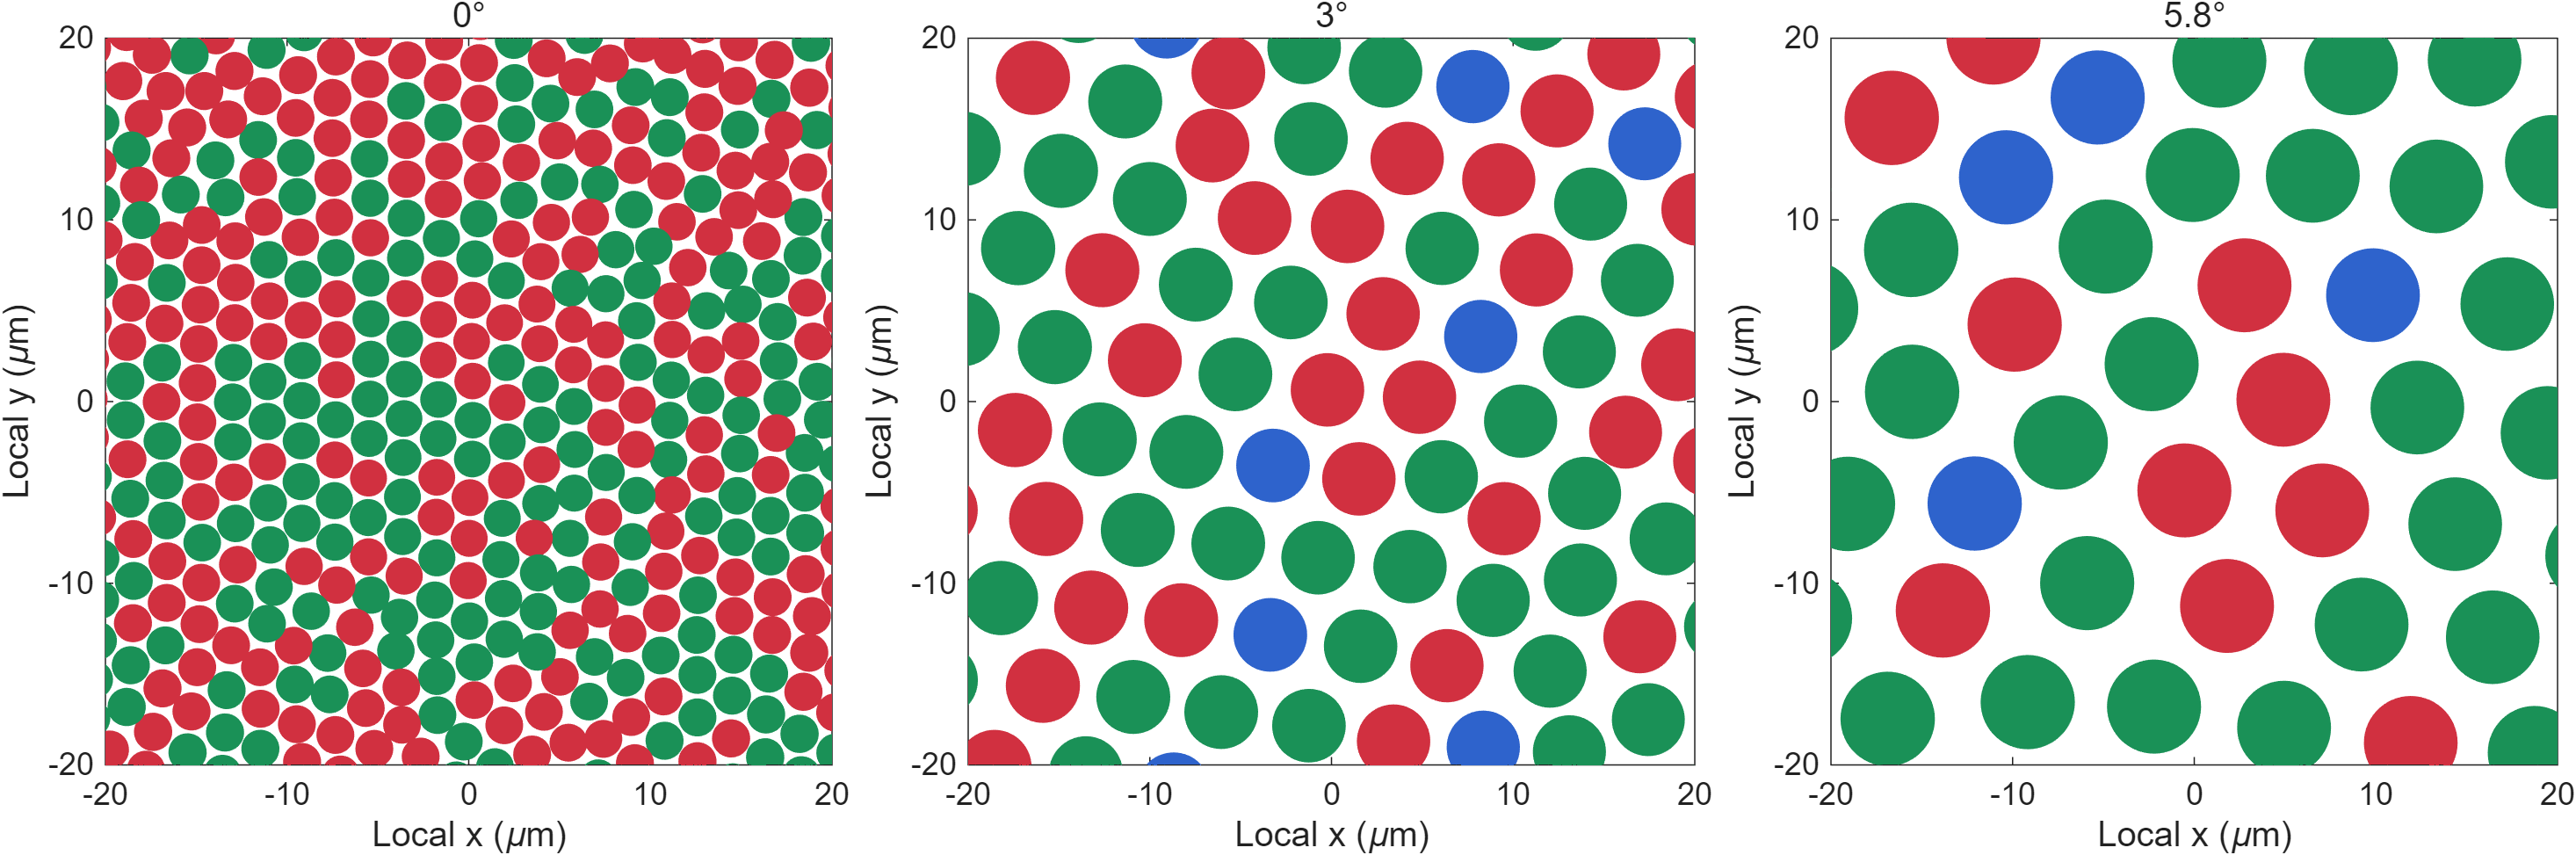
\includegraphics[width=\linewidth]{isetbio_cone_diameter_same_scale.png}\par
\captionof{figure}{Coneの大きさの変化を取り入れた分布生成プレビュー。}
\label{fig:cone-preview}

\begin{center}
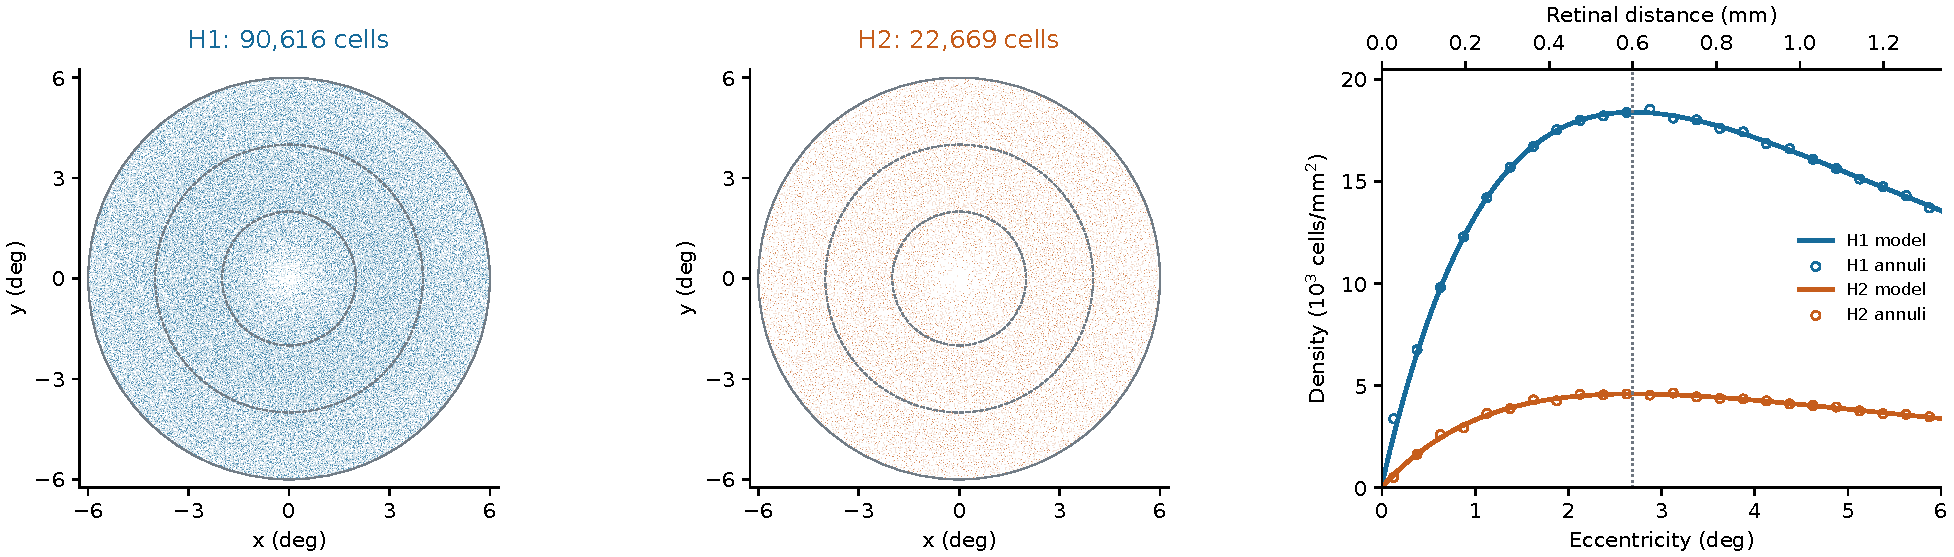
\includegraphics[width=\linewidth]{hc_distribution_density.pdf}
\captionof{figure}{H1/H2細胞体分布と密度。解剖座標の中心から半径$6\degc$相当の範囲に
H1 $90{,}616$個、H2 $22{,}669$個を配置した。
右の実線はモデル密度、白抜き点は保存済み座標の環帯密度を示す。
$6\degc$は$1.338$~mmに相当する。}
\label{fig:mosaic}
\end{center}

\clearpage
\begin{center}
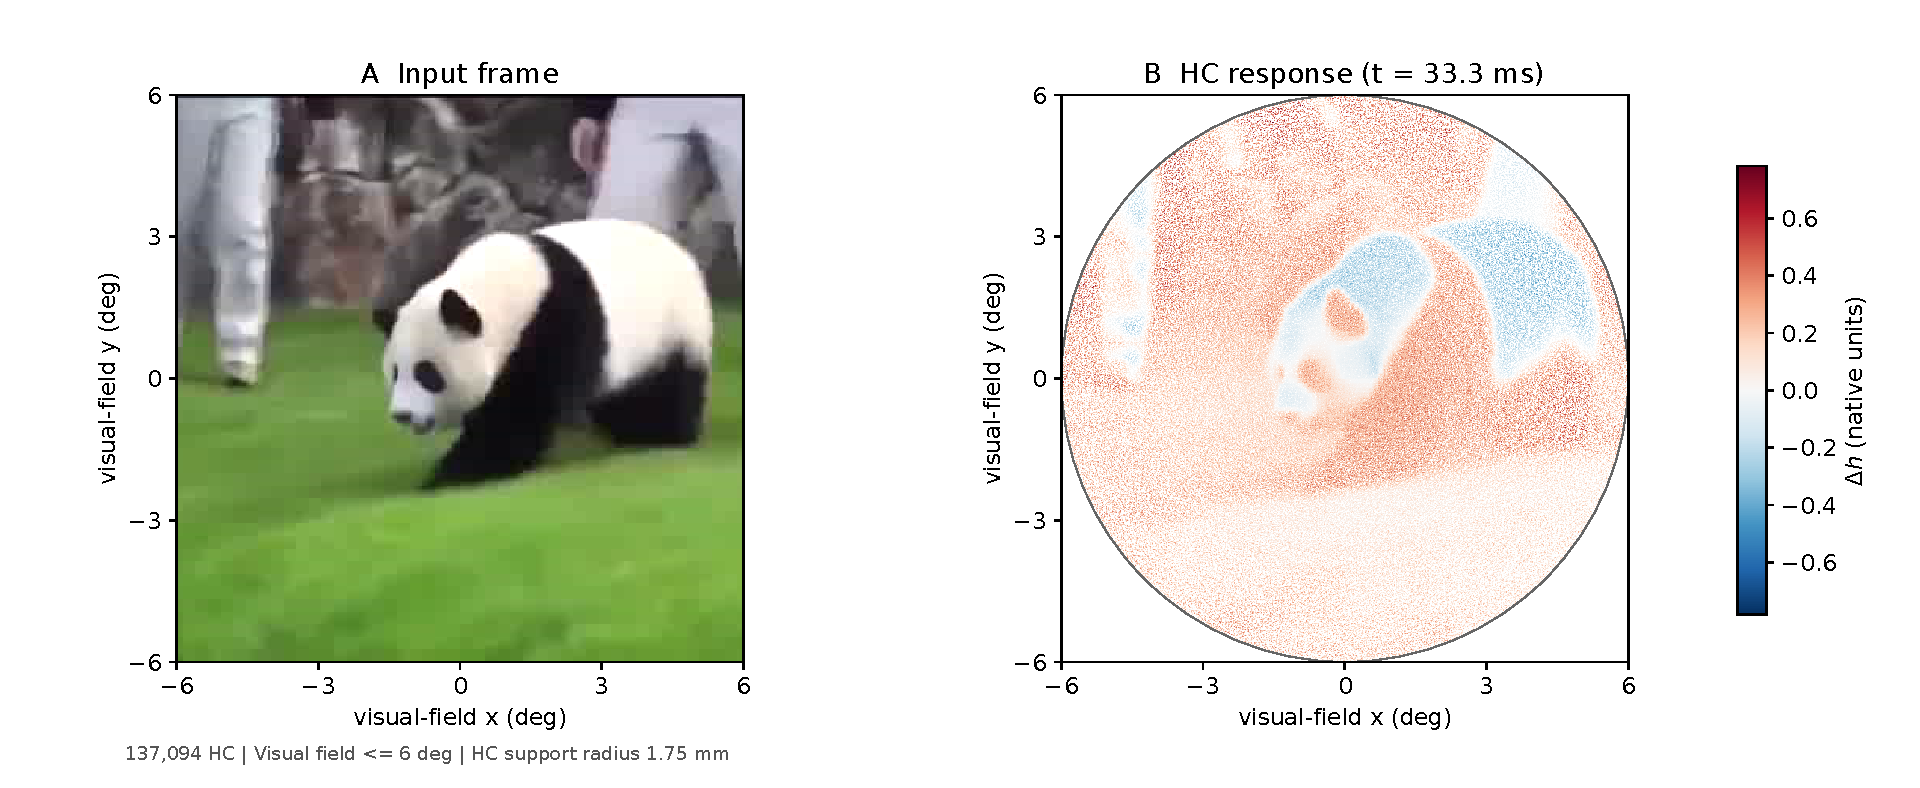
\includegraphics[width=0.8\linewidth]{hc_fullfield_response_preview.pdf}
\captionof{figure}{Coneからの入力に対するHCの応答。}
\label{fig:hc-response-preview}
\end{center}

\begin{center}
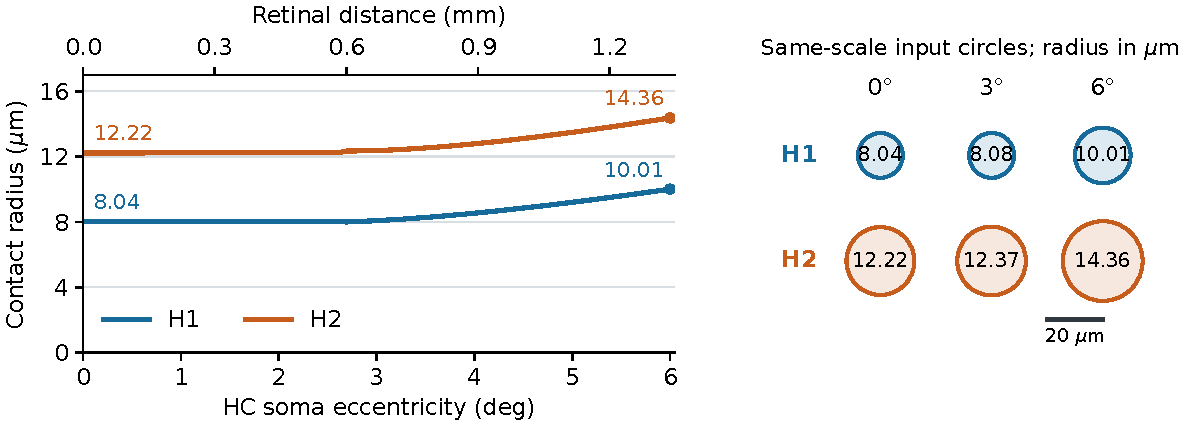
\includegraphics[width=0.95\linewidth]{hc_contact_radius_comparison.pdf}
\captionof{figure}{H1/H2の接触半径（直接Cone入力範囲）の比較。
横軸はHC胞体の偏心度を表す。
Wässleら（1989，2000）とBoycottら（1987）を参考に設定したモデル値を示す\cite{Wassle1989,Wassle2000,Boycott1987}。}
\label{fig:hc-contact-radius}
\end{center}

\section{分布の出典と密度方程式}
\begin{multicols}{2}\small
\subsection{密度とサイズの出典}
密度関数にはVirtual Human Retina（Lyら，2025）の3項指数式の形式を用いた\cite{Ly2025}。
総HC密度のデータはRöhrenbeckら（1989）、KrebsとKrebs（1989）、Ahmadら（2003）を参考にした\cite{Rohrenbeck1989,Krebs1989,Ahmad2003}。
H1/H2の密度と細胞数比、および直接Cone入力範囲の偏心度による変化はWässleら（2000）\cite{Wassle2000}を参考にした。
係数はこれらの文献データを基準に設定した。

\columnbreak
\subsection{密度関数}
偏心度を$e$（度）、物理距離を$r$（mm）とし、
\begin{equation}
r=0.223e
\end{equation}
で換算する。総密度$\rho(r)$（cells/mm$^2$）は、
\begin{align}
\rho(r)={}&45245.3026\,e^{-0.861612866r}\notag\\
&-48597.4424\,e^{-3.112593836r}\notag\\
&+3602.1397\,e^{-0.034949943r}
\end{align}
とした。

HCは上記の密度関数に従って半径$1.75$~mmまで配置し、$0$--$6\degc$視野内のConeが接続する範囲を確保した。
van Hateren（2005）のモデルを用いてHCの応答を生成した\cite{vanHateren2005}。
\end{multicols}

\clearpage
{\footnotesize
\begin{thebibliography}{8}
\setlength{\itemsep}{0pt}
\bibitem{Ly2025}
K. Ly et al.
Virtual human retina: Simulating neural signalling, degeneration, and responses to electrical stimulation.
\textit{Brain Stimulation}, 18(1):144--163, 2025.
\url{https://doi.org/10.1016/j.brs.2025.01.013}.
\bibitem{Rohrenbeck1989}
J. Röhrenbeck, H. Wässle, and B. B. Boycott.
Horizontal Cells in the Monkey Retina: Immunocytochemical staining with antibodies against calcium binding proteins.
\textit{Eur. J. Neurosci.}, 1:407--420, 1989.
\url{https://doi.org/10.1111/j.1460-9568.1989.tb00349.x}.
\bibitem{Krebs1989}
W. Krebs and I. P. Krebs.
Quantitative morphology of the central fovea in the primate retina.
\textit{Am. J. Anat.}, 184(3):225--236, 1989.
\url{https://doi.org/10.1002/aja.1001840306}.
\bibitem{Ahmad2003}
K. M. Ahmad, K. Klug, S. Herr, P. Sterling, and S. Schein.
Cell density ratios in a foveal patch in macaque retina.
\textit{Visual Neuroscience}, 20(2):189--209, 2003.
\url{https://doi.org/10.1017/S0952523803202091}.
\bibitem{Wassle2000}
H. Wässle et al.
The mosaic of horizontal cells in the macaque monkey retina: With a comment on biplexiform ganglion cells.
\textit{Visual Neuroscience}, 17:591--608, 2000.
\url{https://doi.org/10.1017/S0952523800174097}.
\bibitem{Wassle1989}
H. Wässle, B. B. Boycott, and J. Röhrenbeck.
Horizontal cells in the monkey retina: Cone connections and dendritic network.
\textit{Eur. J. Neurosci.}, 1(5):421--435, 1989.
\url{https://doi.org/10.1111/j.1460-9568.1989.tb00350.x}.
\bibitem{Boycott1987}
B. B. Boycott, J. M. Hopkins, and H. G. Sperling.
Cone connections of the horizontal cells of the rhesus monkey's retina.
\textit{Proc. R. Soc. Lond. B}, 229(1257):345--379, 1987.
\url{https://doi.org/10.1098/rspb.1987.0001}.
\bibitem{vanHateren2005}
J. H. van Hateren.
A cellular and molecular model of response kinetics and adaptation in primate cones and horizontal cells.
\textit{J. Vis.}, 5(4), 2005.
\url{https://doi.org/10.1167/5.4.5}.
\end{thebibliography}
}
\end{document}
